\documentclass{beamer}
\usetheme{default}
\usepackage{tikz}
\usetikzlibrary{arrows.meta, positioning, shapes.geometric}

\title{TART Catalogue System Architecture}
\author{Tim Molteno}
\date{\today}

\begin{document}

\begin{frame}{TART Catalogue System Architecture}
\centering

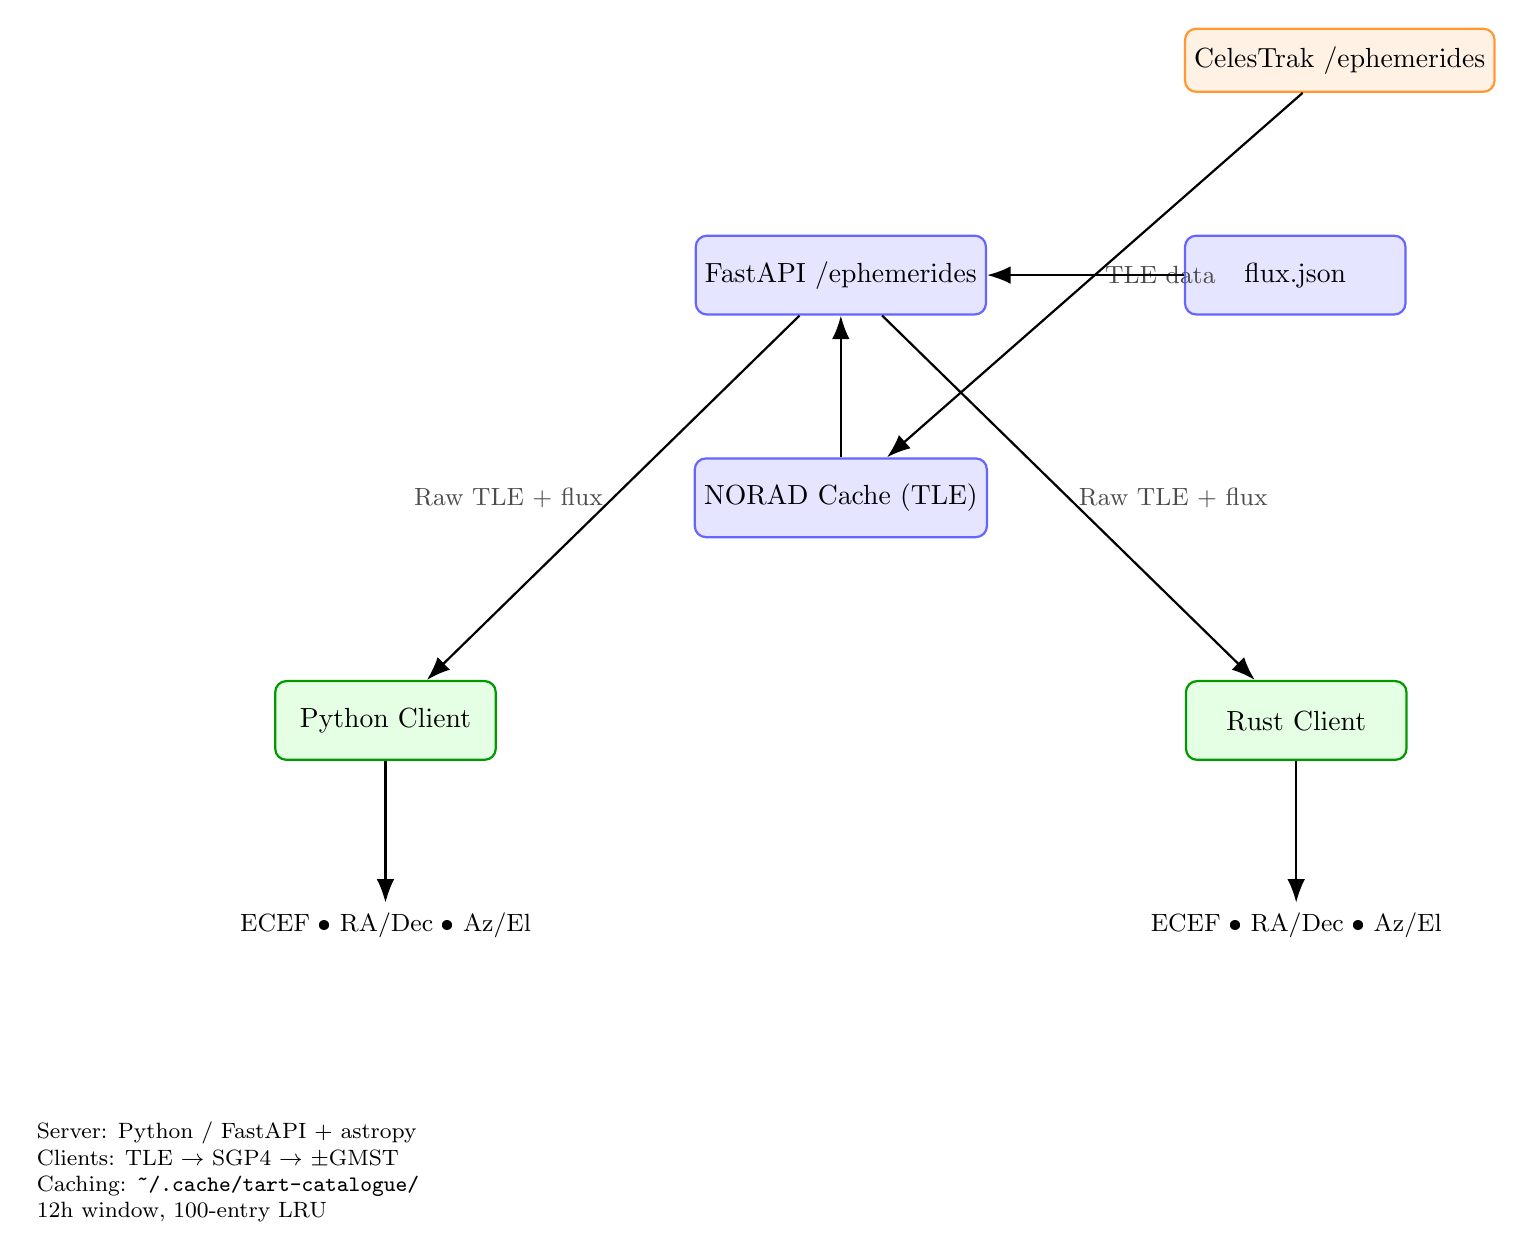
\begin{tikzpicture}[
  node distance=1.8cm and 2.5cm,
  server/.style={rectangle, draw=blue!60, fill=blue!10, thick, minimum width=2.8cm, minimum height=1.0cm, rounded corners},
  client/.style={rectangle, draw=green!60!black, fill=green!10, thick, minimum width=2.8cm, minimum height=1.0cm, rounded corners},
  data/.style={rectangle, draw=orange!80, fill=orange!10, thick, minimum width=2.2cm, minimum height=0.8cm, rounded corners},
  arrow/.style={-{Latex[length=3mm]}, thick},
  label/.style={font=\small, text=gray!60!black},
]

% Top level: external data source
\node[data] (celestrak) {CelesTrak /ephemerides};

% Middle: server components
\node[server, below left=of celestrak] (fastapi) {FastAPI /ephemerides};
\node[server, right=of fastapi] (flux) {flux.json};
\node[server, below=of fastapi] (norad) {NORAD Cache (TLE)};

% Clients
\node[client, below left=of norad] (pyclient) {Python Client};
\node[client, below right=of norad] (rclient) {Rust Client};

% Data flows
\draw[arrow] (celestrak) -- node[label, right] {TLE data} (norad);
\draw[arrow] (norad) -- (fastapi);
\draw[arrow] (flux) -- (fastapi);

\draw[arrow] (fastapi) -- node[label, left] {Raw TLE + flux} (pyclient);
\draw[arrow] (fastapi) -- node[label, right] {Raw TLE + flux} (rclient);

% Client output
\node[below=of pyclient, align=center, font=\small] (pyout) {ECEF \textbullet{} RA/Dec \textbullet{} Az/El};
\node[below=of rclient, align=center, font=\small] (rout) {ECEF \textbullet{} RA/Dec \textbullet{} Az/El};

\draw[arrow] (pyclient) -- (pyout);
\draw[arrow] (rclient) -- (rout);

% Legend
\node[below=of pyout, xshift=-2cm, yshift=-0.3cm, align=left, font=\footnotesize] {
  Server: Python / FastAPI + astropy \\
  Clients: TLE $\to$ SGP4 $\to$ $\pm$GMST \\
  Caching: \texttt{\textasciitilde/.cache/tart-catalogue/} \\
  12h window, 100-entry LRU
};

\end{tikzpicture}

\end{frame}
\end{document}
